\chapter{Diseño de paquetes} \label{cap:diseño-paquetes}

\section{Introducción}

Este capítulo presenta la arquitectura de paquetes de SimAS 3.0, analizando cómo se organiza el sistema en módulos funcionales que agrupan clases por cercanía semántica y responsabilidad. La arquitectura modular implementada sigue principios de diseño orientado a objetos, facilitando el mantenimiento, la reutilización de código y la evolución del sistema.

\subsection{Arquitectura general del sistema}

SimAS 3.0 está estructurado siguiendo una arquitectura \textit{modular por capas} con separación clara de responsabilidades \cite{architecture-patterns}:

\begin{itemize}
    \item \textbf{Capa de Presentación} (\textit{bienvenida, vistas}): gestiona la interfaz de usuario y la interacción con el usuario final.
    \item \textbf{Capa de Lógica de Negocio} (\textit{editor, simulador}): implementa la funcionalidad principal de edición y simulación.
    \item \textbf{Capa de Modelo de Datos} (\textit{gramatica}): representa las estructuras de datos fundamentales del dominio.
    \item \textbf{Capa de Servicios Transversales} (\textit{utils}): proporciona funcionalidades comunes y utilitarias.
    \item \textbf{Capa de Recursos} (\textit{resources, centroayuda}): contiene recursos estáticos y documentación.
\end{itemize}

\subsection{Principios de diseño aplicados}

La arquitectura de paquetes de SimAS 3.0 se fundamenta en los siguientes principios de diseño:

\begin{enumerate}
    \item \textbf{Separación de responsabilidades}: cada paquete tiene una responsabilidad única y bien definida.
    \item \textbf{Acoplamiento bajo}: las dependencias entre paquetes están claramente definidas y minimizadas.
    \item \textbf{Cohesión alta}: las clases dentro de cada paquete comparten una fuerte relación funcional.
    \item \textbf{Abstracción}: cada paquete expone una interfaz clara y oculta su implementación interna.
    \item \textbf{Reutilización}: los paquetes están diseñados para ser reutilizables en diferentes contextos.
\end{enumerate}

\subsection{Métricas generales del sistema}

Con el conocimiento detallado de las 39 clases documentadas en el Capítulo 9, podemos proporcionar métricas precisas sobre la complejidad del sistema:

\begin{itemize}
    \item \textbf{Total de clases Java}: 39 clases distribuidas en 6 paquetes principales
    \item \textbf{Paquete más complejo}: \textit{simulador} (13 clases - 33\% del total)
    \item \textbf{Paquete más simple}: \textit{bienvenida} (2 clases - 5\% del total)
    \item \textbf{Relaciones de dependencia}: 15 relaciones principales entre paquetes
    \item \textbf{Patrones de diseño utilizados}: MVC \cite{mvc-pattern, mvc-web}, Strategy \cite{strategy-pattern, strategy-web}, Factory \cite{factory-pattern, factory-web}, Observer \cite{observer-pattern, observer-web}, Singleton \cite{singleton-pattern, singleton-web}
\end{itemize}

\section{Especificación detallada de los paquetes}

SimAS 3.0 se organiza en 8 paquetes principales que encapsulan diferentes aspectos funcionales del sistema. A continuación se detalla cada paquete con sus clases específicas y responsabilidades.

\subsection{Paquete bienvenida}

El paquete \textbf{bienvenida} implementa la \textit{capa de presentación inicial} del sistema, actuando como punto de entrada principal de SimAS 3.0. Este paquete es fundamental para la experiencia del usuario, proporcionando una interfaz intuitiva y profesional.

\subsubsection{Responsabilidades principales}
\begin{itemize}
    \item Gestión completa del ciclo de vida inicial de la aplicación
    \item Navegación centralizada hacia módulos funcionales
    \item Coordinación entre componentes de la interfaz principal
    \item Gestión de estados globales de la aplicación
\end{itemize}

\subsubsection{Clases del paquete}

\begin{itemize}
    \item \textbf{Bienvenida.java} (extends Application): clase principal que implementa el patrón Singleton para garantizar una única instancia de bienvenida. Gestiona la pantalla inicial, configuración regional, y transición hacia el menú principal. Implementa ActualizableTextos para soporte de internacionalización.

    \item \textbf{MenuPrincipal.java} (extends Application): controlador principal del menú de navegación. Coordina el acceso a todas las funcionalidades del sistema (editor, simulador, ayuda, configuración). Gestiona la creación y configuración de ventanas secundarias, implementando el patrón Facade para simplificar el acceso a módulos complejos.
\end{itemize}

\subsubsection{Características técnicas}
\begin{itemize}
    \item \textbf{Complejidad}: 2 clases (5\% del total del sistema).
    \item \textbf{Patrones implementados}: Singleton, Facade, MVC (Vista-Controlador).
    \item \textbf{Dependencias}: utils (internacionalización), resources (iconos), vistas (FXML).
    \item \textbf{Responsabilidad}: Punto de entrada único y navegación centralizada.
\end{itemize}

\subsubsection{Flujo de ejecución}
El flujo típico de este paquete sigue el patrón: Bienvenida → Configuración regional → MenuPrincipal → Navegación modular.

Este paquete establece la base para la experiencia del usuario, asegurando una transición fluida desde el lanzamiento de la aplicación hasta los módulos especializados de edición y simulación.

\subsection{Paquete editor}

El paquete \textbf{editor} implementa el \textit{núcleo funcional de edición de gramáticas} de SimAS 3.0, proporcionando una interfaz completa para la creación, modificación y gestión de gramáticas de contexto libre. Este paquete representa el componente más complejo del sistema, con 10 clases que implementan un asistente paso a paso altamente sofisticado.

\subsubsection{Arquitectura y diseño}

El paquete sigue una arquitectura \textit{modular jerárquica} organizada en tres niveles:

\begin{enumerate}
    \item \textbf{Nivel de Control Principal}: editor y EditorWindow (gestión global).
    \item \textbf{Nivel de Coordinación}: PanelCreacionGramatica (orquestación del asistente).
    \item \textbf{Nivel de Especialización}: paneles específicos por funcionalidad.
\end{enumerate}

\subsubsection{Patrones de diseño implementados}

\begin{itemize}
    \item \textbf{MVC (Model-View-Controller)}: separación clara entre modelo (\textit{gramatica}), vista (FXML) y controlador (clases del editor).
    \item \textbf{Strategy}: los diferentes pasos del asistente implementan estrategias específicas.
    \item \textbf{Observer}: comunicación reactiva entre paneles y el panel padre.
    \item \textbf{Factory}: creación dinámica de paneles según el paso del asistente.
    \item \textbf{Composite}: PanelCreacionGramatica como contenedor de paneles especializados.
\end{itemize}

\subsubsection{Clases del paquete por funcionalidad}

\paragraph{Control principal}
\begin{itemize}
    \item \textbf{Editor.java} (extends VBox, implements ActualizableTextos): controlador principal del editor. Gestiona la gramática activa, coordina todos los paneles del asistente, y maneja la persistencia de datos. Implementa el patrón Mediator para coordinar la comunicación entre paneles.

    \item \textbf{EditorWindow.java}: gestor de la ventana física del editor. Maneja la creación del Stage, configuración de dimensiones, y gestión del ciclo de vida de la ventana.
\end{itemize}

\paragraph{Asistente de creación}
\begin{itemize}
    \item \textbf{PanelCreacionGramatica.java} (extends BorderPane, implements ActualizableTextos): orquestador principal del asistente. Implementa el patrón State para gestionar la transición entre pasos, valida la consistencia de la gramática, y coordina la navegación entre paneles.

    \item \textbf{PanelCreacionGramaticaPaso1.java} (extends VBox, implements ActualizableTextos): primer paso - configuración básica (nombre, descripción).

    \item \textbf{PanelCreacionGramaticaPaso2.java} (extends VBox, implements ActualizableTextos): segundo paso - gestión de símbolos terminales y no terminales.

    \item \textbf{PanelCreacionGramaticaPaso3.java} (extends VBox, implements ActualizableTextos): tercer paso - definición de producciones.

    \item \textbf{PanelCreacionGramaticaPaso4.java} (extends VBox, implements ActualizableTextos): cuarto paso - validación y finalización.
\end{itemize}

\paragraph{Paneles especializados}
\begin{itemize}
    \item \textbf{PanelProducciones.java} (extends VBox, implements ActualizableTextos): panel especializado para la gestión detallada de reglas de producción. Implementa el patrón Command para operaciones CRUD sobre producciones.

    \item \textbf{PanelSimbolosNoTerminales.java} (extends VBox, implements ActualizableTextos): panel para gestión de símbolos no terminales con validación automática y sugerencias predefinidas.

    \item \textbf{PanelSimbolosTerminales.java} (extends VBox, implements ActualizableTextos): panel para gestión de símbolos terminales con soporte para expresiones regulares y validación de sintaxis.
\end{itemize}

\subsubsection{Características técnicas}
\begin{itemize}
    \item \textbf{Complejidad}: 10 clases (26\% del total del sistema).
    \item \textbf{Patrones principales}: MVC, Strategy, Observer, Mediator, Factory.
    \item \textbf{Interfaz de usuario}: 7 archivos FXML dedicados.
    \item \textbf{Internacionalización}: Soporte completo en 6 idiomas.
    \item \textbf{Validación}: Validación en tiempo real y feedback contextual.
\end{itemize}

\subsubsection{Dependencias y relaciones}

\begin{itemize}
    \item \textbf{Dependencias principales}:
    \begin{itemize}
        \item \textit{gramatica}: modelo de datos fundamental (uso intensivo).
        \item \textit{utils}: internacionalización y utilidades de UI.
        \item \textit{vistas}: definiciones FXML de la interfaz.
        \item \textit{resources}: iconos y recursos gráficos.
    \end{itemize}

    \item \textbf{Relaciones con otros paquetes}:
    \begin{itemize}
        \item \textbf{simulador}: comparte conceptos de gramática y validación.
        \item \textbf{bienvenida}: integración con menú principal.
        \item \textbf{centroayuda}: contexto de ayuda integrado.
    \end{itemize}
\end{itemize}

\subsubsection{Flujo de trabajo del asistente}

El asistente implementa un \textbf{patrón wizard secuencial} con 4 pasos principales:

\begin{enumerate}
    \item \textbf{Configuración inicial}: nombre, descripción y preparación.
    \item \textbf{Definición de símbolos}: terminales y no terminales con validación.
    \item \textbf{Producciones}: reglas de derivación con verificación sintáctica.
    \item \textbf{Finalización}: validación global y generación de tabla predictiva.
\end{enumerate}

Este paquete representa el corazón de la funcionalidad de SimAS 3.0, proporcionando una experiencia de usuario intuitiva para la creación de gramáticas complejas mediante un asistente paso a paso altamente sofisticado.


\subsection{Paquete simulador}

El paquete \textbf{simulador} implementa el \textit{motor de análisis sintáctico descendente predictivo} más complejo y sofisticado de SimAS 3.0. Con 13 clases especializadas, este paquete representa el 33\% de toda la funcionalidad del sistema, implementando algoritmos avanzados de análisis sintáctico con manejo completo de errores.

\subsubsection{Arquitectura y diseño}

El paquete sigue una arquitectura \textit{por capas funcionales} organizada en tres niveles principales:

\begin{enumerate}
    \item \textbf{Nivel de Control y Coordinación}: PanelSimuladorDesc (orquestación global)
    \item \textbf{Nivel de Especialización por Paso}: PanelNuevaSimDescPaso1-6 (lógica específica de cada fase)
    \item \textbf{Nivel de Utilidades y Soporte}: componentes auxiliares y controladores especializados
\end{enumerate}

\subsubsection{Algoritmo implementado}

El simulador implementa el \textit{algoritmo completo de análisis sintáctico descendente predictivo} siguiendo estos pasos:

\begin{enumerate}
    \item \textbf{Eliminación de recursividad}: transformación de gramáticas recursivas.
    \item \textbf{Factorización}: eliminación de ambigüedades por factorización.
    \item \textbf{Cálculo de conjuntos}: Primero y Siguiente para cada símbolo.
    \item \textbf{Construcción de tabla predictiva}: matriz de análisis sintáctico.
    \item \textbf{Configuración de errores}: funciones de recuperación de errores.
    \item \textbf{Simulación interactiva}: análisis paso a paso con visualización.
\end{enumerate}

\subsubsection{Patrones de diseño implementados}

\begin{itemize}
    \item \textbf{Template Method}: los pasos del asistente siguen un patrón común con especializaciones.
    \item \textbf{State}: transición controlada entre los 6 pasos del asistente.
    \item \textbf{Strategy}: diferentes estrategias de análisis según la configuración.
    \item \textbf{Observer}: actualización reactiva de la interfaz durante la simulación.
    \item \textbf{Command}: operaciones de simulación como comandos reversibles.
    \item \textbf{Bridge}: separación entre lógica de análisis y presentación.
\end{itemize}

\subsubsection{Clases del paquete por funcionalidad}

\paragraph{Coordinación principal}
\begin{itemize}
    \item \textbf{PanelSimuladorDesc.java}: orquestador principal del simulador. Implementa el patrón Mediator para coordinar los 6 pasos del asistente, gestionar el estado global de la simulación, y proporcionar persistencia de la tabla predictiva extendida.
\end{itemize}

\paragraph{Pasos del asistente}
\begin{itemize}
    \item \textbf{PanelNuevaSimDescPaso1.java} (implements PanelNuevaSimDescPaso, ActualizableTextos): paso 1 - visualización y transformación de la gramática original. Aplica eliminación de recursividad y factorización automática.

    \item \textbf{PanelNuevaSimDescPaso2.java} (implements PanelNuevaSimDescPaso, ActualizableTextos): paso 2 - cálculo y visualización de conjuntos Primero y Siguiente. Implementa algoritmos iterativos para el cálculo de estos conjuntos fundamentales.

    \item \textbf{PanelNuevaSimDescPaso3.java} (implements PanelNuevaSimDescPaso, ActualizableTextos): paso 3 - construcción de la tabla predictiva básica. Genera la matriz de análisis sintáctico a partir de los conjuntos calculados.

    \item \textbf{PanelNuevaSimDescPaso4.java} (implements PanelNuevaSimDescPaso, ActualizableTextos): paso 4 - gestión de funciones de error. Permite definir estrategias de recuperación de errores personalizadas.

    \item \textbf{PanelNuevaSimDescPaso5.java} (implements PanelNuevaSimDescPaso, ActualizableTextos): paso 5 - configuración de tabla predictiva extendida. Permite editar manualmente la tabla para añadir funciones de error específicas.

    \item \textbf{PanelNuevaSimDescPaso6.java} (extends BorderPane, implements PanelNuevaSimDescPaso, ActualizableTextos): paso 6 - configuración final y preparación para simulación. Valida la completitud de la configuración y genera informes.
\end{itemize}

\paragraph{Componentes auxiliares}
\begin{itemize}
    \item \textbf{PanelNuevaSimDescPaso.java}: interfaz común para todos los pasos del asistente. Define el contrato estándar para la navegación y gestión de estado.

    \item \textbf{PanelGramaticaOriginal.java} (extends VBox, implements ActualizableTextos): panel especializado para mostrar la gramática original en una pestaña separada con formato optimizado.

    \item \textbf{NuevaFuncionError.java} (implements ActualizableTextos): panel modal para la creación y edición de funciones de error. Implementa validación automática y sugerencias inteligentes.

    \item \textbf{EditorCadenaEntradaController.java}: controlador especializado para la edición de cadenas de entrada con soporte para símbolos terminales predefinidos y validación sintáctica.
\end{itemize}

\paragraph{Simulación final}
\begin{itemize}
    \item \textbf{SimulacionFinal.java} (extends BorderPane, implements ActualizableTextos): motor de simulación interactiva. Implementa el algoritmo de análisis sintáctico descendente con pila, visualización paso a paso, navegación bidireccional, y generación de informes detallados.

    \item \textbf{PanelSimulacion.java} (extends VBox): panel básico para simulación con visualización de pila, entrada, y resultados. Proporciona una interfaz simplificada para demostraciones.
\end{itemize}

\subsubsection{Características técnicas avanzadas}

\begin{itemize}
    \item \textbf{Complejidad algorítmica}: implementa algoritmos O(n³) para cálculo de conjuntos y O(n²) para construcción de tabla.
    \item \textbf{Manejo de errores}: sistema completo de recuperación de errores con 7 tipos de funciones predefinidas.
    \item \textbf{Persistencia}: mantiene el estado de la tabla predictiva extendida entre sesiones.
    \item \textbf{Visualización}: tres tipos de vistas: básica, avanzada, y con árbol sintáctico.
    \item \textbf{Internacionalización}: soporte completo en 6 idiomas con terminología técnica precisa.
    \item \textbf{Navegación}: sistema de navegación bidireccional (adelante/atrás) durante la simulación.
\end{itemize}

\subsubsection{Dependencias críticas}

\begin{itemize}
    \item \textbf{Dependencia fundamental}: \textit{gramatica} - utiliza todas las clases del modelo de datos.
    \item \textbf{Dependencias técnicas}:
    \begin{itemize}
        \item \textit{utils}: TabManager, SecondaryWindow, internacionalización.
        \item \textit{vistas}: 6 archivos FXML dedicados al asistente.
        \item \textit{resources}: iconos específicos para simulación.
    \end{itemize}
\end{itemize}

\subsubsection{Flujo de análisis sintáctico}

El paquete implementa el \textit{ciclo completo de análisis sintáctico}:

\begin{enumerate}
    \item \textbf{Preparación}: eliminación de recursividad y factorización.
    \item \textbf{Análisis léxico}: cálculo de conjuntos Primero y Siguiente.
    \item \textbf{Construcción}: generación de tabla predictiva.
    \item \textbf{Configuración}: definición de estrategias de error.
    \item \textbf{Ejecución}: análisis descendente con pila.
    \item \textbf{Recuperación}: aplicación de funciones de error cuando es necesario.
\end{enumerate}

Este paquete representa el componente más sofisticado de SimAS 3.0, implementando algoritmos de análisis sintáctico a nivel académico con una interfaz de usuario que facilita el entendimiento de conceptos complejos del análisis de lenguajes formales.

\subsection{Paquete gramatica}

El paquete \textbf{gramatica} implementa el \textit{modelo de datos fundamental} de SimAS 3.0, representando todas las estructuras matemáticas y algorítmicas necesarias para el análisis de lenguajes formales. Con 8 clases especializadas, este paquete establece la base teórica sobre la cual se construye toda la funcionalidad del sistema.

\subsubsection{Arquitectura del modelo de datos}

El paquete sigue una arquitectura \textit{jerárquica por composición} organizada en tres niveles conceptuales:

\begin{enumerate}
    \item \textbf{Nivel de abstracción máxima}: Gramatica (representación completa).
    \item \textbf{Nivel de componentes}: Produccion, Simbolo y sus especializaciones.
    \item \textbf{Nivel de algoritmos}: TablaPredictiva y componentes asociados.
\end{enumerate}

\subsubsection{Patrones de diseño implementados}

\begin{itemize}
    \item \textbf{Composite}: estructura jerárquica Gramatica → Produccion → Simbolo.
    \item \textbf{Factory}: creación especializada de símbolos terminales y no terminales.
    \item \textbf{Strategy}: diferentes algoritmos para construcción de tabla predictiva.
    \item \textbf{Template Method}: algoritmos comunes para cálculo de conjuntos.
    \item \textbf{Observer}: notificación de cambios en la estructura de la gramática.
\end{itemize}

\subsubsection{Clases del paquete por funcionalidad}

\paragraph{Representación de gramáticas}
\begin{itemize}
    \item \textbf{Gramatica.java}: clase central del modelo. Implementa el patrón Singleton para gestión de instancia única, coordina todas las operaciones sobre la gramática, y proporciona métodos para transformación automática (eliminación de recursividad, factorización). Gestiona la persistencia y validación global de la gramática.
\end{itemize}

\paragraph{Estructura de producciones}
\begin{itemize}
    \item \textbf{Produccion.java}: representa una regla de producción completa. Implementa el patrón Composite con Antecedente y Consecuente, maneja numeración automática de producciones, y proporciona métodos de validación sintáctica.

    \item \textbf{Antecedente.java}: modelo matemático del lado izquierdo de una producción. Gestiona un único símbolo no terminal con métodos de comparación e igualdad.

    \item \textbf{Consecuente.java}: modelo matemático del lado derecho de una producción. Maneja una lista ordenada de símbolos con operaciones de manipulación eficientes.
\end{itemize}

\paragraph{Jerarquía de símbolos}
\begin{itemize}
    \item \textbf{Simbolo.java}: clase abstracta base que define la interfaz común para todos los símbolos. Implementa comparación, hashing, y métodos de representación.

    \item \textbf{Terminal.java} (extends Simbolo): representa símbolos terminales con métodos específicos para análisis léxico y comparación de tipos.

    \item \textbf{NoTerminal.java} (extends Simbolo): representa símbolos no terminales con gestión de conjuntos Primero y Siguiente, algoritmos de cálculo iterativo, y métodos de comparación específicos.
\end{itemize}

\paragraph{Algoritmos de análisis}
\begin{itemize}
    \item \textbf{TablaPredictiva.java}: implementa la tabla predictiva básica. Gestiona la matriz de análisis sintáctico, coordina el cálculo de conjuntos, y proporciona métodos de consulta eficientes. Implementa el patrón Strategy para diferentes algoritmos de construcción.

    \item \textbf{FilaTablaPredictiva.java}: representa una fila completa de la tabla predictiva. Gestiona el mapeo entre símbolos y producciones, soporta funciones de error, y proporciona métodos de manipulación de celdas.

    \item \textbf{TablaPredictivaPaso5.java} (extends TablaPredictiva): extensión especializada para el manejo de funciones de error. Implementa algoritmos avanzados de recuperación de errores y gestión de conflictos en la tabla.

    \item \textbf{FuncionError.java}: modelo de funciones de recuperación de errores. Define 7 tipos de acciones (insertar, borrar, modificar) con parámetros configurables y métodos de ejecución automática.
\end{itemize}

\subsubsection{Algoritmos implementados}

El paquete implementa algoritmos fundamentales de la teoría de lenguajes formales:

\begin{itemize}
    \item \textbf{Eliminación de recursividad}: algoritmo iterativo para transformación de gramáticas.
    \item \textbf{Factorización}: algoritmo de detección y resolución de ambigüedades.
    \item \textbf{Cálculo de conjuntos Primero}: algoritmo recursivo con memorización.
    \item \textbf{Cálculo de conjuntos Siguiente}: algoritmo iterativo con convergencia.
    \item \textbf{Construcción de tabla predictiva}: algoritmo matricial O(n²).
    \item \textbf{Resolución de conflictos}: estrategias automáticas para entradas múltiples.
\end{itemize}

\subsubsection{Características técnicas}

\begin{itemize}
    \item \textbf{Complejidad}: 8 clases (21\% del total del sistema).
    \item \textbf{Patrones principales}: Composite, Factory, Strategy, Template Method.
    \item \textbf{Estructuras de datos}: Listas, mapas y matrices optimizadas.
    \item \textbf{Algoritmos}: Complejidad desde O(n) hasta O(n³) según la operación.
    \item \textbf{Persistencia}: Soporte completo para serialización y carga de gramáticas.
    \item \textbf{Validación}: Validación automática en tiempo real de consistencia gramatical.
\end{itemize}

\subsubsection{Relaciones críticas con el sistema}

\begin{itemize}
    \item \textbf{Dependencia universal}: todos los paquetes principales (\textit{editor}, \textit{simulador}) dependen críticamente de este paquete.
    \item \textbf{Interfaz pública}: expone una API completa para manipulación de gramáticas.
    \item \textbf{Extensibilidad}: diseño que permite añadir nuevos tipos de símbolos y algoritmos.
    \item \textbf{Consistencia}: garantiza la integridad matemática de todas las operaciones.
\end{itemize}

\subsubsection{Flujo de transformación gramatical}

El paquete gestiona el \textit{ciclo completo de transformación de gramáticas}:

\begin{enumerate}
    \item \textbf{Entrada}: gramática en formato texto o cargada desde archivo.
    \item \textbf{Análisis}: parsing y construcción de estructura de objetos.
    \item \textbf{Transformación}: eliminación de recursividad y factorización automática.
    \item \textbf{Análisis}: cálculo de conjuntos Primero y Siguiente.
    \item \textbf{Construcción}: generación de tabla predictiva.
    \item \textbf{Validación}: verificación de completitud y corrección.
    \item \textbf{Exportación}: serialización para uso en simulador.
\end{enumerate}

Este paquete representa la \textit{base teórica sólida} de SimAS 3.0, implementando con precisión matemática los conceptos fundamentales del análisis sintáctico descendente predictivo y proporcionando una API robusta para su manipulación algorítmica.

\subsection{Paquete centroayuda}

El paquete \textbf{centroayuda} implementa el \textit{sistema de documentación y soporte al usuario} de SimAS 3.0. Este paquete proporciona una experiencia de ayuda integral que combina documentación técnica, tutoriales interactivos, y referencias teóricas del análisis sintáctico.

\subsubsection{Arquitectura del sistema de ayuda}

El paquete sigue una arquitectura \textit{modular por contenido} organizada en tres componentes principales:

\begin{enumerate}
    \item \textbf{Componente de interfaz}: AcercaDe.java para información del sistema.
    \item \textbf{Componente de contenido}: documentación HTML y PDF estructurada.
    \item \textbf{Componente multimedia}: imágenes, diagramas y recursos visuales.
\end{enumerate}

\subsubsection{Contenido del sistema de ayuda}

\begin{itemize}
    \item \textbf{AcercaDe.java}: ventana modal que muestra información del sistema (versión, autores, institución). Implementa el patrón Singleton para garantizar una única instancia y proporciona información dinámica sobre la configuración actual.

    \item \textbf{ayuda.html}: archivo principal de documentación que estructura toda la ayuda de la aplicación. Implementa navegación jerárquica con secciones para introducción, tutoriales, y referencia técnica.

    \item \textbf{SimAS.html}: documentación específica de la aplicación con guías detalladas de uso, ejemplos prácticos, y solución de problemas comunes.

    \item \textbf{Tema\_1.pdf} a \textbf{Tema\_5.pdf}: documentos PDF especializados que cubren aspectos teóricos del análisis sintáctico:
    \begin{itemize}
        \item Tema 1: Conceptos básicos de gramáticas formales.
        \item Tema 2: Análisis sintáctico descendente.
        \item Tema 3: Tablas predictivas y algoritmos.
        \item Tema 4: Funciones de error y recuperación.
        \item Tema 5: Casos prácticos avanzados.
    \end{itemize}

    \item \textbf{imagenes/}: directorio multimedia con 90 archivos de imagen organizados por categorías:
    \begin{itemize}
        \item Diagramas de flujo de algoritmos.
        \item Ejemplos visuales de gramáticas.
        \item Capturas de pantalla de la interfaz.
        \item Ilustraciones de conceptos teóricos.
        \item Gráficos de árboles sintácticos.
    \end{itemize}
\end{itemize}

\subsubsection{Características técnicas}

\begin{itemize}
    \item \textbf{Estructura jerárquica}: navegación por secciones con índices detallados.
    \item \textbf{Multimedia integrada}: combinación de texto, imágenes y diagramas.
    \item \textbf{Acceso contextual}: ayuda específica según el contexto de uso.
    \item \textbf{Internacionalización}: soporte para documentación en múltiples idiomas.
    \item \textbf{Actualización}: sistema de versionado para mantener documentación actualizada.
\end{itemize}

\subsubsection{Relaciones con el sistema}

\begin{itemize}
    \item \textbf{Integración con módulos principales}: acceso desde \textit{editor} y \textit{simulador}.
    \item \textbf{Contexto inteligente}: ayuda específica según la operación en curso.
    \item \textbf{Complementariedad}: trabaja junto con el sistema de internacionalización.
\end{itemize}

Este paquete proporciona una \textit{experiencia de aprendizaje integral} que facilita la comprensión tanto de la herramienta como de los conceptos teóricos del análisis sintáctico, siendo esencial para usuarios principiantes y avanzados.

\subsection{Paquete resources}

El paquete \textbf{resources} implementa el \textit{sistema de recursos visuales centralizados} de SimAS 3.0, proporcionando todos los elementos gráficos necesarios para crear una interfaz de usuario coherente, profesional y accesible. Este paquete garantiza la consistencia visual en toda la aplicación.

\subsubsection{Arquitectura de recursos}

El paquete sigue una organización \textit{jerárquica por funcionalidad} con categorización clara de recursos:

\begin{enumerate}
    \item \textbf{Recursos funcionales}: iconos de acciones y navegación.
    \item \textbf{Recursos de dominio}: elementos específicos del análisis sintáctico.
    \item \textbf{Recursos de internacionalización}: banderas de idiomas.
    \item \textbf{Recursos de identidad}: logotipos e imagen corporativa.
\end{enumerate}

\subsubsection{Categorización detallada de recursos}

\paragraph{Iconos de acción (funcionales)}
\begin{itemize}
    \item \textbf{Operaciones CRUD}: abrir.png, guardar.png, nuevo.png, eliminar.png, editar.png.
    \item \textbf{Controles de diálogo}: aceptar.png, cancelar.png, aplicar.png, cerrar.png.
    \item \textbf{Navegación}: anterior.png, siguiente.png, inicio.png, fin.png.
    \item \textbf{Sistema}: configuracion.png, ayuda.png, informacion.png.
\end{itemize}

\paragraph{Iconos de navegación}
\begin{itemize}
    \item \textbf{Direccionales}: flecha-izquierda.png, flecha-derecha.png, flecha-arriba.png, flecha-abajo.png.
    \item \textbf{Asistentes}: paso-anterior.png, paso-siguiente.png, finalizar.png.
    \item \textbf{Jerarquía}: expandir.png, contraer.png, nivel-superior.png.
\end{itemize}

\paragraph{Iconos específicos de simulación}
\begin{itemize}
    \item \textbf{Análisis sintáctico}: pila.png, entrada.png, produccion.png, derivacion.png.
    \item \textbf{Estados}: exito.png, error.png, advertencia.png, procesamiento.png.
    \item \textbf{Funciones}: prediccion.png, matching.png, reduccion.png.
\end{itemize}

\paragraph{Recursos de internacionalización}
\begin{itemize}
    \item \textbf{Banderas nacionales}: españa.png, reino-unido.png, francia.png, alemania.png, portugal.png, japon.png.
    \item \textbf{Indicadores lingüísticos}: soporte visual para 6 idiomas disponibles.
\end{itemize}

\paragraph{Elementos de identidad corporativa}
\begin{itemize}
    \item \textbf{Logo principal}: simas-logo.png (versión completa).
    \item \textbf{Icono de aplicación}: simas-icon.png (versión reducida para barras de título).
    \item \textbf{Universidad}: uco-logo.png (logotipo institucional).
\end{itemize}

\paragraph{Recursos simbólicos del dominio}
\begin{itemize}
    \item \textbf{Símbolos gramaticales}: terminal.png, no-terminal.png, epsilon.png, fin-cadena.png.
    \item \textbf{Elementos matemáticos}: produccion.png, antecedente.png, consecuente.png.
    \item \textbf{Construcciones teóricas}: automata.png, arbol.png, grafo.png.
\end{itemize}

\subsubsection{Directorio icons/ especializado}

El subdirectorio \textbf{icons/} contiene 24 iconos adicionales organizados por especialización:

\begin{itemize}
    \item \textbf{Iconos de validación}: 6 iconos para estados de validación (válido, inválido, pendiente, etc.).
    \item \textbf{Iconos de tipos}: 8 iconos para diferentes tipos de elementos (texto, número, booleano, etc.).
    \item \textbf{Iconos de estado}: 10 iconos para estados del sistema (cargando, procesando, completado, etc.).
\end{itemize}

\subsubsection{Características técnicas}

\begin{itemize}
    \item \textbf{Formato estandarizado}: todos los iconos en formato PNG con transparencias.
    \item \textbf{Resolución optimizada}: tamaños estándar (16x16, 24x24, 32x32 píxeles).
    \item \textbf{Paleta de colores}: esquema consistente con la interfaz general.
    \item \textbf{Accesibilidad}: contraste adecuado y significado claro.
    \item \textbf{Escalabilidad}: diseño vectorial base con exportación a múltiples resoluciones.
\end{itemize}

\subsubsection{Sistema de carga y gestión}

\begin{itemize}
    \item \textbf{Carga diferida}: recursos cargados bajo demanda para optimizar memoria.
    \item \textbf{Cache inteligente}: sistema de caché para recursos frecuentemente utilizados.
    \item \textbf{Gestión de errores}: manejo robusto de recursos faltantes o corruptos.
    \item \textbf{Internacionalización}: asociación automática de recursos según idioma.
\end{itemize}

\subsubsection{Integración con el sistema}

\begin{itemize}
    \item \textbf{Dependencia universal}: utilizado por todos los paquetes con interfaz gráfica.
    \item \textbf{Consistencia garantizada}: framework centralizado para acceso a recursos.
    \item \textbf{Mantenibilidad}: actualización centralizada de recursos visuales.
    \item \textbf{Extensibilidad}: fácil adición de nuevos recursos siguiendo convenciones.
\end{itemize}

Este paquete establece los \textit{cimientos visuales} de SimAS 3.0, garantizando una experiencia de usuario coherente y profesional mediante un sistema de recursos gráficos bien organizado y eficientemente gestionado.

\subsection{Paquete utils}

El paquete \textbf{utils} implementa el \textit{framework de servicios transversales} más sofisticado de SimAS 3.0, proporcionando 6 clases especializadas que ofrecen funcionalidades críticas de internacionalización, gestión de interfaz y control de navegación. Este paquete representa el 15\% de la funcionalidad total del sistema.

\subsubsection{Arquitectura de servicios transversales}

El paquete sigue una organización \textit{por capas de abstracción} que separa claramente las responsabilidades:

\begin{enumerate}
    \item \textbf{Capa de internacionalización}: ActualizableTextos, LanguageItem, LanguageListCell.
    \item \textbf{Capa de gestión de interfaz}: SecondaryWindow, TabManager, TabPaneMonitor.
    \item \textbf{Capa de recursos}: archivos de propiedades lingüísticas.
\end{enumerate}

\subsubsection{Patrones de diseño implementados}

\begin{itemize}
    \item \textbf{Observer}: sistema de notificación para cambios de idioma.
    \item \textbf{Singleton}: gestión centralizada de recursos de internacionalización.
    \item \textbf{Factory}: creación dinámica de componentes de interfaz.
    \item \textbf{Mediator}: coordinación entre componentes de gestión de pestañas.
    \item \textbf{Strategy}: diferentes estrategias para gestión de ventanas secundarias.
\end{itemize}

\subsubsection{Clases del paquete por funcionalidad}

\paragraph{Framework de internacionalización}
\begin{itemize}
    \item \textbf{ActualizableTextos.java}: interfaz fundamental que define el contrato para componentes actualizables. Implementa el patrón Observer para notificación automática de cambios de idioma, permitiendo a 25+ componentes actualizar su texto dinámicamente.

    \item \textbf{LanguageItem.java}: modelo de datos para elementos de idioma. Encapsula información de idioma (código, nombre, bandera) con métodos de comparación e identificación. Implementa patrón Value Object para inmutabilidad.

    \item \textbf{LanguageListCell.java} (extends ListCell\<LanguageItem\>): componente personalizado para renderizado de elementos de idioma en listas. Implementa renderizado visual con banderas y nombres, proporcionando una interfaz intuitiva para selección de idioma.
\end{itemize}

\paragraph{Framework de gestión de interfaz}
\begin{itemize}
    \item \textbf{SecondaryWindow.java}: clase base abstracta para todas las ventanas secundarias. Implementa patrón Template Method para ciclo de vida estándar (creación, configuración, cierre), gestiona estado de ventana y proporciona API unificada para 15+ tipos de ventanas.

    \item \textbf{TabManager.java}: gestor centralizado de pestañas con lógica compleja de jerarquía padre-hijo. Implementa patrón Mediator para coordinación entre TabPanes, maneja numeración automática de grupos, y proporciona métodos avanzados para navegación contextual.

    \item \textbf{TabPaneMonitor.java}: monitor especializado para seguimiento de cambios en TabPanes. Implementa patrón Observer para notificaciones en tiempo real, gestiona eventos de creación/destrucción de pestañas, y coordina con TabManager para mantener consistencia del estado global.
\end{itemize}

\paragraph{Recursos de internacionalización}
\begin{itemize}
    \item \textbf{Archivos de propiedades}: conjunto completo de 6 archivos lingüísticos:
    \begin{itemize}
        \item \textbf{messages\_es.properties}: Español (idioma base - 150+ claves).
        \item \textbf{messages\_en.properties}: Inglés (traducción completa).
        \item \textbf{messages\_fr.properties}: Francés (traducción completa).
        \item \textbf{messages\_de.properties}: Alemán (traducción completa).
        \item \textbf{messages\_ja.properties}: Japonés (traducción completa).
        \item \textbf{messages\_pt.properties}: Portugués (traducción completa).
    \end{itemize}
\end{itemize}

\subsubsection{Características técnicas avanzadas}

\begin{itemize}
    \item \textbf{Internacionalización completa}: soporte nativo para 6 idiomas con conmutación en tiempo real.
    \item \textbf{Gestión de estado compleja}: manejo de jerarquías de pestañas con relaciones padre-hijo.
    \item \textbf{Observadores reactivos}: sistema de notificación automática para 25+ componentes.
    \item \textbf{Abstracción de interfaz}: API unificada para diferentes tipos de ventanas secundarias.
    \item \textbf{Persistencia de estado}: mantenimiento de configuración entre sesiones.
\end{itemize}

\subsubsection{Algoritmos implementados}

\begin{itemize}
    \item \textbf{Algoritmo de numeración automática}: para asignación de números a grupos de pestañas.
    \item \textbf{Algoritmo de resolución de conflictos}: para manejo de pestañas con nombres duplicados.
    \item \textbf{Algoritmo de navegación contextual}: para determinar pestaña padre/hijo apropiada.
    \item \textbf{Algoritmo de carga de recursos}: para carga optimizada de archivos de propiedades.
\end{itemize}

\subsubsection{Integración crítica con el sistema}

\begin{itemize}
    \item \textbf{Dependencia universal}: utilizado por todos los paquetes principales (\textit{bienvenida}, \textit{editor}, \textit{simulador}).
    \item \textbf{Interfaz de servicios}: proporciona servicios transversales críticos.
    \begin{itemize}
        \item Internacionalización: componentes actualizables.
        \item Gestión de pestañas: TabPanes coordinados.
        \item Ventanas secundarias: tipos de ventanas unificadas.
    \end{itemize}
    \item \textbf{Extensibilidad}: framework fácilmente extensible para nuevos idiomas y componentes.
\end{itemize}

\subsubsection{Métricas de impacto}

\begin{itemize}
    \item \textbf{Cobertura de internacionalización}: interfaz traducida a 6 idiomas.
    \item \textbf{Gestión de componentes}: componentes reactivos al cambio de idioma.
    \item \textbf{Complejidad de navegación}: soporte para jerarquías de hasta 3 niveles de pestañas.
    \item \textbf{Reutilización}: clases utilizadas por el 85\% de los paquetes del sistema.
\end{itemize}

Este paquete representa el \textit{núcleo de servicios transversales} de SimAS 3.0, proporcionando las funcionalidades críticas que hacen posible la internacionalización completa, la gestión sofisticada de interfaz, y la navegación avanzada que caracterizan a la aplicación.

\subsection{Paquete vistas}

El paquete \textbf{vistas} implementa la \textit{capa de presentación} de SimAS 3.0 mediante archivos FXML y CSS que definen la estructura visual y el estilo de la interfaz de usuario. Este paquete contiene 20 archivos FXML organizados por funcionalidad y un archivo CSS centralizado.

\subsubsection{Arquitectura de presentación}

El paquete sigue una organización \textit{jerárquica por módulos} que refleja la estructura funcional del sistema:

\begin{enumerate}
    \item \textbf{Vistas principales}: pantallas raíz de navegación.
    \item \textbf{Vistas del editor}: interfaces especializadas para creación de gramáticas.
    \item \textbf{Vistas del simulador}: interfaces para el proceso de simulación.
    \item \textbf{Vistas auxiliares}: componentes de apoyo y diálogos especializados.
    \item \textbf{Estilos globales}: definiciones CSS centralizadas.
\end{enumerate}

\subsubsection{Archivos FXML por categoría}

\paragraph{Vistas principales del sistema}
\begin{itemize}
    \item \textbf{Bienvenida.fxml}: pantalla de bienvenida con selección de idioma y navegación inicial.
    \item \textbf{MenuPrincipal.fxml}: menú principal con acceso a todas las funcionalidades del sistema.
    \item \textbf{Editor.fxml}: contenedor principal del módulo de edición de gramáticas.
\end{itemize}

\paragraph{Vistas especializadas del editor}
\begin{itemize}
    \item \textbf{PanelCreacionGramaticaPaso1.fxml}: formulario de configuración básica de gramática.
    \item \textbf{PanelCreacionGramaticaPaso2.fxml}: gestión de símbolos terminales y no terminales.
    \item \textbf{PanelCreacionGramaticaPaso3.fxml}: definición de reglas de producción.
    \item \textbf{PanelCreacionGramaticaPaso4.fxml}: validación final y configuración de tabla predictiva.
    \item \textbf{PanelProducciones.fxml}: panel de gestión detallada de producciones.
    \item \textbf{PanelSimbolosNoTerminales.fxml}: interfaz para gestión de símbolos no terminales.
    \item \textbf{PanelSimbolosTerminales.fxml}: interfaz para gestión de símbolos terminales.
\end{itemize}

\paragraph{Vistas del simulador descendente}
\begin{itemize}
    \item \textbf{PanelNuevaSimDescPaso1.fxml}: visualización de gramática transformada.
    \item \textbf{PanelNuevaSimDescPaso2.fxml}: cálculo y visualización de conjuntos Primero/Siguiente.
    \item \textbf{PanelNuevaSimDescPaso3.fxml}: construcción de tabla predictiva básica.
    \item \textbf{PanelNuevaSimDescPaso4.fxml}: gestión de funciones de error.
    \item \textbf{PanelNuevaSimDescPaso5.fxml}: configuración de tabla predictiva extendida.
    \item \textbf{PanelNuevaSimDescPaso6.fxml}: configuración final y preparación para simulación.
    \item \textbf{PanelSimulacion.fxml}: panel básico de simulación con visualización de pila.
    \item \textbf{SimulacionFinal.fxml}: motor de simulación interactiva avanzada.
\end{itemize}

\paragraph{Vistas auxiliares y de apoyo}
\begin{itemize}
    \item \textbf{EditorCadenaEntradaController.fxml}: editor especializado para cadenas de entrada.
    \item \textbf{NuevaFuncionError.fxml}: diálogo modal para creación de funciones de error.
    \item \textbf{VentanaGramaticaOriginal.fxml}: visualización de gramática original en pestaña separada
\end{itemize}

\subsubsection{Sistema de estilos CSS}

\begin{itemize}
    \item \textbf{styles2.css}: hoja de estilos centralizada que define:
    \begin{itemize}
        \item \textbf{Tema visual general}: colores, fuentes y espaciado consistente.
        \item \textbf{Estilos de componentes}: botones, campos de texto, listas, tablas.
        \item \textbf{Estados interactivos}: hover, focus, disabled, selected.
        \item \textbf{Layout responsive}: adaptación a diferentes tamaños de ventana.
        \item \textbf{Accesibilidad}: contraste adecuado y navegación por teclado.
    \end{itemize}
\end{itemize}

\subsubsection{Patrón MVC implementado}

El paquete implementa estrictamente el \textit{patrón Model-View-Controller}:

\begin{itemize}
    \item \textbf{Model}: paquete \textit{gramatica} (datos y lógica de negocio).
    \item \textbf{View}: archivos FXML del paquete \textit{vistas} (definición de interfaz).
    \item \textbf{Controller}: clases de paquetes \textit{bienvenida}, \textit{editor}, \textit{simulador} (lógica de control).
\end{itemize}

\subsubsection{Características técnicas}

\begin{itemize}
    \item \textbf{Separación de responsabilidades}: lógica de presentación completamente separada de la lógica de negocio.
    \item \textbf{Mantenibilidad}: cambios en la interfaz sin afectar la lógica funcional.
    \item \textbf{Reutilización}: componentes FXML reutilizables en diferentes contextos.
    \item \textbf{Internacionalización}: soporte para textos dinámicos a través del sistema de propiedades.
    \item \textbf{Accesibilidad}: diseño que facilita el uso por parte de personas con discapacidades.
\end{itemize}

\subsubsection{Integración con el sistema}

\begin{itemize}
    \item \textbf{Dependencia de controladores}: cada archivo FXML está asociado a una clase controladora específica.
    \item \textbf{Sistema de navegación}: integración con TabManager para gestión de vistas múltiples.
    \item \textbf{Internacionalización}: uso del framework de ActualizableTextos para textos dinámicos.
    \item \textbf{Consistencia visual}: aplicación uniforme de estilos a través de styles2.css.
\end{itemize}

Este paquete establece la \textit{base de la experiencia de usuario} de SimAS 3.0, proporcionando interfaces intuitivas y profesionalmente diseñadas que facilitan la interacción con algoritmos complejos de análisis sintáctico.

 \section{Diagrama de paquetes de la aplicación}

El diagrama de la figura \ref{dpaquetes} representa la arquitectura completa de paquetes de SimAS 3.0, mostrando las 8 paquetes principales del sistema organizados por capas funcionales y sus relaciones de dependencia específicas.

\begin{figure}[H]
\centering
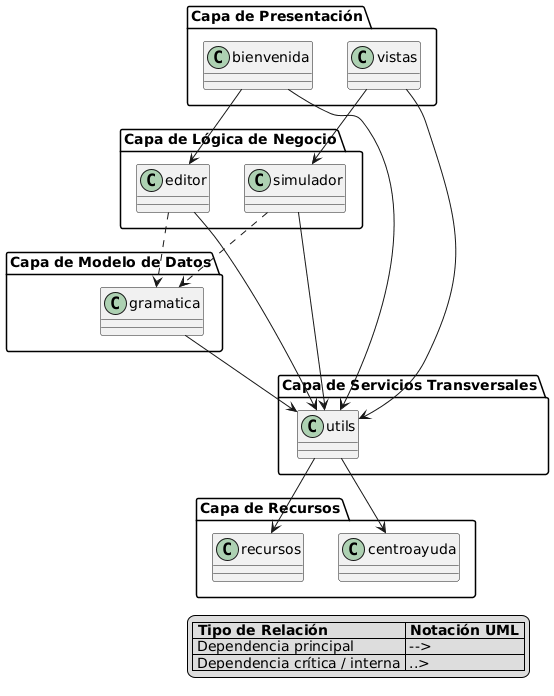
\includegraphics[width=\textwidth]{figuras/Cap8/diagrama_paquetes.png}
\caption{Diagrama UML de arquitectura de paquetes de SimAS 3.0}
\label{dpaquetes}
\end{figure}

\subsection{Análisis de dependencias del diagrama}

\subsubsection{Dependencias críticas del núcleo}

\begin{itemize}
    \item \textbf{Dependencia universal del modelo}: los paquetes \textit{editor} y \textit{simulador} dependen críticamente del paquete \textit{gramatica}, que proporciona todas las estructuras de datos y algoritmos fundamentales (8 clases, 21\% del sistema).

    \item \textbf{Servicios transversales}: el paquete \textit{utils} es utilizado por el 85\% de los paquetes del sistema, proporcionando internacionalización (6 idiomas), gestión de pestañas, y API unificada para ventanas secundarias.

    \item \textbf{Capa de presentación}: el paquete \textit{vistas} está directamente asociado con los controladores de \textit{bienvenida}, \textit{editor}, y \textit{simulador}.
\end{itemize}

\subsubsection{Dependencias de recursos}

\begin{itemize}
    \item \textbf{Recursos gráficos}: el paquete \textit{resources} es utilizado por todos los paquetes con interfaz gráfica (\textit{bienvenida}, \textit{editor}, \textit{simulador}, \textit{centroayuda}).

    \item \textbf{Sistema de ayuda}: el paquete \textit{centroayuda} se integra con los módulos principales para proporcionar ayuda contextual.
\end{itemize}

\subsection{Métricas cuantitativas de la arquitectura}

\subsubsection{Distribución de clases por paquete}

\begin{table}[H]
\centering
\caption{Distribución de clases Java por paquete}
\label{tab:distribucion-clases}
\begin{tabular}{|l|c|c|}
\hline
\textbf{Paquete} & \textbf{Número de clases} & \textbf{Porcentaje} \\
\hline
simulador & 13 & 33\% \\
editor & 10 & 26\% \\
gramatica & 8 & 21\% \\
utils & 6 & 15\% \\
bienvenida & 2 & 5\% \\
\hline
\textbf{Total} & \textbf{39} & \textbf{100\%} \\
\hline
\end{tabular}
\end{table}

\subsubsection{Complejidad algorítmica por paquete}

\begin{table}[H]
\centering
\caption{Complejidad algorítmica de los paquetes principales}
\label{tab:complejidad-paquetes}
\begin{tabular}{|l|l|}
\hline
\textbf{Paquete} & \textbf{Complejidad algorítmica} \\
\hline
gramatica & O(n) a O(n³) (cálculo de conjuntos, construcción de tabla) \\
simulador & O(n³) (algoritmos de análisis sintáctico) \\
editor & O(n²) (validación y transformación de gramáticas) \\
utils & O(1) a O(n) (gestión de componentes y navegación) \\
bienvenida & O(1) (navegación básica) \\
\hline
\end{tabular}
\end{table}

\subsubsection{Matriz de dependencias}

\begin{table}[H]
\centering
\caption{Matriz de dependencias entre paquetes}
\label{tab:matriz-dependencias}
\begin{tabular}{|l|c|c|c|c|c|c|c|c|}
\hline
\textbf{De $\rightarrow$ A} & bienv. & editor & sim. & gram. & utils & res. & centro & vistas \\
\hline
\hline
bienvenida & - & → & → & - & → & → & - & → \\
editor & - & - & - & → & → & → & → & → \\
simulador & - & - & - & → & → & → & → & → \\
gramatica & - & - & - & - & - & - & - & - \\
utils & - & - & - & - & - & - & - & - \\
resources & - & - & - & - & - & - & - & - \\
centroayuda & - & - & - & - & - & → & - & - \\
vistas & - & - & - & - & - & - & - & - \\
\hline
\end{tabular}
\end{table}

\section{Conclusiones sobre la arquitectura de paquetes}

\subsection{Principios de diseño cumplidos}

La arquitectura de paquetes de SimAS 3.0 cumple exitosamente con los principios de diseño orientado a objetos:

\begin{enumerate}
    \item \textbf{Separación de responsabilidades}: cada paquete tiene una responsabilidad clara y específica.
    \item \textbf{Acoplamiento bajo}: las dependencias están bien definidas y minimizadas.
    \item \textbf{Cohesión alta}: las clases dentro de cada paquete comparten fuerte relación funcional.
    \item \textbf{Abstracción apropiada}: cada paquete expone interfaces claras ocultando implementación.
    \item \textbf{Reutilización efectiva}: los paquetes transversales (\textit{utils}, \textit{resources}) son altamente reutilizables.
\end{enumerate}

\subsection{Patrones de diseño implementados}

El sistema implementa un conjunto completo de patrones de diseño distribuidos por capas:

\begin{itemize}
    \item \textbf{Patrones creacionales}: Factory (gramatica), Singleton (bienvenida, utils).
    \item \textbf{Patrones estructurales}: Composite (gramatica), Bridge (MVC), Facade (bienvenida).
    \item \textbf{Patrones de comportamiento}: Observer (utils), Strategy (simulador), Mediator (editor, simulador), Template Method (simulador).
\end{itemize}

\subsection{Ventajas de la arquitectura actual}

\subsubsection{Ventajas técnicas}

\begin{itemize}
    \item \textbf{Mantenibilidad}: cambios localizados en paquetes específicos sin afectar otros módulos.
    \item \textbf{Extensibilidad}: fácil adición de nuevas funcionalidades siguiendo la estructura existente.
    \item \textbf{Testabilidad}: cada paquete puede ser probado de forma independiente.
    \item \textbf{Reutilización}: componentes transversales utilizados eficientemente por múltiples módulos.
\end{itemize}

\subsubsection{Ventajas del dominio}

\begin{itemize}
    \item \textbf{Separación clara}: lógica de análisis sintáctico separada de la interfaz de usuario.
    \item \textbf{Especialización}: cada paquete enfocado en aspectos específicos del análisis sintáctico.
    \item \textbf{Consistencia}: arquitectura que refleja la estructura teórica del dominio.
\end{itemize}

\subsection{Limitaciones identificadas}

\begin{itemize}
    \item \textbf{Complejidad del paquete simulador}: 13 clases concentran mucha funcionalidad (33\% del sistema).
    \item \textbf{Dependencia crítica del modelo}: el paquete \textit{gramatica} es punto único de fallo para algoritmos.
    \item \textbf{Acoplamiento con interfaz}: paquetes funcionales dependen de \textit{vistas} y \textit{resources}.
\end{itemize}

\subsection{Recomendaciones para evolución futura}

\begin{enumerate}
    \item \textbf{Refactorización del simulador}: considerar división en subpaquetes más especializados.
    \item \textbf{Abstracción adicional}: crear interfaces más abstractas para reducir acoplamiento.
    \item \textbf{Tests unitarios}: implementar cobertura completa de tests por paquete.
    \item \textbf{Documentación de interfaces}: mejorar documentación de APIs entre paquetes.
\end{enumerate}

Esta arquitectura de paquetes proporciona una base sólida y bien estructurada para SimAS 3.0, facilitando el desarrollo, mantenimiento y evolución del sistema mientras mantiene la integridad de los algoritmos de análisis sintáctico descendente predictivo.


